\chapter{Methodology II: VLM Supervision and the Trustworthiness Wrapper (the Headline)}
\label{ch:vlm-wrapper}

The preceding chapter specified the \emph{engine}: a frozen DINOv2 ViT-S/14
backbone feeding five per--action-unit (AU) CORN ordinal heads, decoded to
per-AU levels in $\{0,1,2\}$, summed to a $0$--$10$ Feline Grimace Scale (FGS)
total, and thresholded at the $0.39$ analgesia cut. That engine is conceded
throughout as \emph{plumbing}: it is assembled from standard, off-the-shelf
components and is never claimed as a novel contribution. The present chapter is
where the contribution of this work actually lives. It specifies (i) the
weak-supervision pipeline by which a vision--language model (VLM) produces the
ordinal per-AU labels that the engine consumes, and (ii) the
\emph{trustworthiness wrapper} --- the frame in which the system's outputs are
reported, audited, and gated.

Two of the components below are designated \textbf{portable methods}: they are
dataset-agnostic protocols, released as runnable code, that any future
facial-pain-scoring corpus can re-run. These are the headline deliverables of
the project:

\begin{enumerate}
  \item \textbf{Headline Method 1 --- VLM-as-AU-rater $\kappa$
  (\S\ref{sec:vlm-au-rater-kappa}).} A measurement of whether a frozen VLM can
  weak-label feline FGS action units at human-rater agreement, expressed as five
  per-AU quadratic-weighted kappas against a veterinary anchor, gated on the
  \emph{confidence-interval lower bound} (Gate~1-B).
  \item \textbf{Headline Method 2 --- capture-condition confound-attribution
  protocol (\S\ref{sec:confound-protocol}).} A one-directional audit
  (\emph{FGS-BG-Gap} plus per-AU energy-based pointing game, EBPG) that detects
  whether the scorer is reading acquisition context rather than grimace.
\end{enumerate}

Between these sit the wrapper pillars --- a welfare-asymmetric decision curve, a
fixed-high-sensitivity operating point, and a defer-to-vet abstention boundary
reported as a one-sided lower bound --- which together constitute the clinical
framing that distinguishes this work from a generic pain detector.

\paragraph{Status of this chapter.} This is a methodology and evaluation
protocol. No experiment has yet been run. Every quantitative claim in this
chapter is stated as a \emph{protocol} together with the \emph{decision rule}
(the gate) it feeds; where the literature is cited (e.g.\ Evangelista et al.\ on
human-rater FGS agreement), the numbers are attributed to that source and are
not results of this project. Figures that depend on data not yet collected are
presented as captioned schematic placeholders or as TikZ process diagrams ---
never as plots of invented measurements.

\section{The VLM weak-labeling pipeline}
\label{sec:vlm-pipeline}

The supervision problem is structural. The only in-domain corpus
(\S\ref{ch:datasets}) carries binary \texttt{pain}/\texttt{no\_pain} boxes and
\emph{zero} per-AU or $0$--$10$ FGS labels; no open graded cat-FGS dataset
exists. The five per-AU ordinal targets that the CORN engine requires must
therefore be \emph{manufactured} at low cost and then anchored against a small
veterinary gold set. The weak labeler is a frozen, hosted VLM (Claude),
prompted to emit five FGS action-unit scores per face under a strict,
machine-checkable contract.

\subsection{Forced-tool-use enum schema, rationale-before-score}
\label{sec:vlm-schema}

The VLM is constrained to a single forced tool call. Each of the five AUs is a
nested object whose ordinal level is an \texttt{enum} over $[0,1,2]$ ---
strict structured-output decoding strips numeric \texttt{min}/\texttt{max}
constraints, so an enumeration is the only reliable way to pin the three ordinal
levels. The tool is invoked with
\texttt{tool\_choice=\{"type":"tool",\dots\}} and
\texttt{disable\_parallel\_tool\_use=true} so that exactly one tool-use block is
emitted; \texttt{additionalProperties:false} and an all-\texttt{required} field
set make any contract violation a hard parse failure rather than a silent
mislabel. Within each AU object the \texttt{rationale} field is ordered
\emph{before} the \texttt{score} field, because under tool-use generation the
JSON-schema property order is the token-generation order: the model is forced to
articulate the visible feature before committing to a level. Each AU also
carries a \texttt{confidence} enum (\texttt{low}/\texttt{medium}/\texttt{high})
and an \texttt{abstain} boolean (set when the AU region is occluded, blurred,
out-of-frame, or non-frontal), and the call carries a whole-face
\texttt{image\_quality} enum
(\texttt{frontal\_clear}/\texttt{partial}/\texttt{unusable}).

Crucially, the schema contains \textbf{no \texttt{sum} field, no
\texttt{decision} field, and no \texttt{pain} field}. These quantities are
uncomputable by the VLM \emph{by construction}: the labeler emits five atoms in
$\{0,1,2\}$ and nothing else. The total and the $0.39$ flag are computed in code
(\S\ref{sec:vlm-aggregation}), so the threshold definition has a single source
of truth in the repository and the labeler cannot leak a clinical decision it
was never validated to make.

\begin{figure}[t]
\centering
\begin{tikzpicture}[
  node distance=6mm and 12mm,
  box/.style={draw, rounded corners, align=center, inner sep=4pt, font=\small},
  au/.style={draw, align=center, inner sep=3pt, font=\footnotesize, fill=black!4},
  code/.style={draw, rounded corners, align=center, inner sep=4pt, font=\small, fill=black!8},
  ban/.style={draw, dashed, align=center, inner sep=3pt, font=\footnotesize},
  >=latex
]
\node[box] (img) {cat face crop\\(518$\times$518, frontal)};
\node[box, right=of img] (vlm) {frozen VLM\\forced single tool call\\\texttt{tool\_choice=tool}};
\node[au, right=20mm of vlm, yshift=20mm] (ear)   {ear: rationale $\to$ \texttt{enum[0,1,2]}};
\node[au, below=2mm of ear]  (orb)   {orbital: rationale $\to$ \texttt{enum[0,1,2]}};
\node[au, below=2mm of orb]  (muz)   {muzzle: rationale $\to$ \texttt{enum[0,1,2]}};
\node[au, below=2mm of muz]  (whi)   {whiskers: rationale $\to$ \texttt{enum[0,1,2]}};
\node[au, below=2mm of whi]  (hea)   {head: rationale $\to$ \texttt{enum[0,1,2]}};
\node[code, below=14mm of vlm] (agg) {in-code aggregation\\sum $\in\{0,\dots,10\}$\\flag $=\,\mathbb{1}[\,\text{sum}/10\geq 0.39\,]$};
\node[ban, below=6mm of hea] (noban) {\textbf{NOT in schema:}\\no \texttt{sum}, no \texttt{decision}, no \texttt{pain}};

\draw[->] (img) -- (vlm);
\draw[->] (vlm.east) -- (ear.west);
\draw[->] (vlm.east) -- (orb.west);
\draw[->] (vlm.east) -- (muz.west);
\draw[->] (vlm.east) -- (whi.west);
\draw[->] (vlm.east) -- (hea.west);
\draw[->] (muz.south west) .. controls +(left:8mm) and +(right:8mm) .. (agg.east);
\draw[->, dashed] (noban) -- (hea);
\end{tikzpicture}
\caption[Forced-tool-use enum schema]{The forced-tool-use enum schema. The VLM
emits five per-AU records, each \emph{rationale-before-score} over an ordinal
\texttt{enum[0,1,2]}; the $0$--$10$ sum and the $0.39$ analgesia flag are
computed \emph{in code}, never by the VLM. The schema contains no total and no
decision field by construction, so the labeler cannot emit a clinical decision.}
\label{fig:vlm-schema}
\end{figure}

\subsection{The frozen Evangelista rubric in a cached system block}
\label{sec:vlm-rubric}

The scoring rubric is a system block containing one paragraph per AU using the
verbatim Evangelista et al.\ ordinal descriptors~\cite{evangelista2019}
($0=$ absent; $1=$ moderately present or uncertain; $2=$
marked/obvious), with the AU anatomy grounded in CatFACS. The block instructs
the model to \emph{default genuine ambiguity to level~1 with low confidence},
and to set \texttt{abstain} on any occluded, blurred, or non-frontal AU region.
This block is byte-frozen and carried with \texttt{cache\_control} so that the
full corpus run pays for the rubric once; any byte change invalidates the cache,
and the cache hash is pinned in the run configuration for reproducibility (the
run logs \texttt{cache\_read\_input\_tokens}$>0$ to confirm a cache hit). The
frontal-pose and quality gate is thus \emph{inside} the schema rather than a
separate model: \texttt{image\_quality} and per-AU \texttt{abstain} route
non-frontal or occluded crops to the veterinary queue, which the abstention
curve (\S\ref{sec:abstention}) later consumes as a counted channel rather than a
silent drop.

\subsection{Bulk execution: the Message Batches API}
\label{sec:vlm-batch}

The full-corpus weak-labeling run is executed through the Message Batches API
(asynchronous, with a substantial cost discount), sharing the single cached
rubric block across all requests. One request is built per image; a
self-consistency subset is run $N\geq 3$ times at raised temperature to support
the ordinal Krippendorff $\alpha$ axis (\S\ref{sec:vlm-consistency}). The bulk
run is \emph{blocked} until the kappa pilot (Gate~1-B,
\S\ref{sec:vlm-au-rater-kappa}) returns \textsc{go}; on \textsc{no-go} the
project pivots to the binary-plus-wrapper fallback and the kappa numbers ship as
a method finding regardless. All of this section is hosted-API-only --- no local
VLM weights --- so it is identical on the Apple~M4 development machine or any
cloud worker.

\subsection{In-code aggregation: the sum and the $0.39$ flag}
\label{sec:vlm-aggregation}

The five emitted atoms are summed in code to a total $s\in\{0,\dots,10\}$, and
the analgesia flag is $\mathbb{1}[\,s/10 \geq 0.39\,]$ (the Evangelista
$\geq 4/10$ cut~\cite{evangelista2019}). \textbf{This is the identical decode
contract pinned by the engine's blocking Gate~4 unit test}
(decode $\to$ per-AU $0$--$2$ $\to$ sum $\to$ $0.39$): the VLM path and the CORN
path must produce identical sums from identical five-atom inputs, and both
import the same aggregation function, so there is exactly one threshold
definition in the repository. The flag here is \emph{decision-support triage
only}, never an autonomous analgesia trigger, and the sum it rides on is an
\emph{inspected-not-validated} quantity. Following the project-wide honesty
constraint, the word ``graded'' is struck from every validated-claim sentence.

\subsection{Vet-free self-consistency: ordinal Krippendorff $\alpha$}
\label{sec:vlm-consistency}

A vet-free reliability axis runs each image of the self-consistency subset
$N\geq 3$ times at raised temperature and computes the \emph{ordinal}
Krippendorff~$\alpha$~\cite{krippendorff2004} per AU over the
runs-$\times$-items matrix. This serves three purposes: a cheap pre-screen
before any veterinary budget is spent; an abstention signal (low-$\alpha$ AUs
route to vet); and a complement to --- never a replacement for --- the
against-vet kappa of \S\ref{sec:vlm-au-rater-kappa}. Low $\alpha$ on muzzle and
whiskers is anticipated: these are among the weakest AUs even for human experts,
and that expectation feeds both the abstention curve and the per-AU confidence
gating. Self-consistency $\alpha$ is never offered as validation of the $0.39$
flag (\S\ref{sec:firewall}).

\section{Headline Method 1: VLM-as-AU-rater kappa}
\label{sec:vlm-au-rater-kappa}

The first portable contribution is a \emph{measurement}: can a frozen VLM
weak-label feline FGS action units at human-rater agreement? The deliverable is
the \emph{protocol plus result} --- released code that scores any face corpus's
per-AU VLM labels against a veterinary anchor and reports five quadratic kappas
with confidence-interval lower bounds. The numbers obtained on the present
corpus instantiate the protocol; they are not its point. This is the one
fact-about-the-world the project produces, and it is immune to the
``routine hygiene'' critique precisely because no prior feline-pain work has
measured it.

\subsection{The veterinary anchor and the review loop}
\label{sec:vet-anchor}

The anchor is the project's single source of trustworthy per-AU $0/1/2$ labels.
It is not downloaded --- it is \emph{produced} by a prefilled review loop: the
VLM scores each crop with rationale-before-score; the cases that buy the most
information per veterinary hour are triaged to the top (pain-positive and
near-threshold cases with sum $3$--$5/10$; the weakest AUs, muzzle and whiskers;
the most-diagnostic orbital-tightening AU; confident-learning
error flags~\cite{cleanlab2021}; and multi-run VLM disagreements); and the
veterinarian \emph{accepts or corrects} the prefilled scores rather than
labeling from a blank slate. Only vet-confirmed rows enter the kappa
computation. The anchor size is not guessed: it is the single integer fixed by
the Gate~0 power calculation (a $\kappa$ CI half-width target of $\leq 0.15$ via
\texttt{kappaSize}) before any veterinary hour is spent.

\subsection{Per-AU quadratic-weighted kappa, gated on the CI lower bound}
\label{sec:kappa-gate}

For each AU, agreement is the quadratic-weighted Cohen kappa~\cite{cohen1968kappa}
between the VLM level and the vet level, computed row-paired with
\texttt{weights="quadratic"}. The quadratic weighting is what makes the statistic
\emph{ordinal} --- it penalizes a $0$-versus-$2$ disagreement four times as
heavily as a $0$-versus-$1$ disagreement --- and is the difference between a
nominal agreement number and a contribution-grade ordinal one. A one-sided
$95\%$ \emph{lower bound} on each per-AU kappa is obtained by case-resampling
bootstrap (degenerate single-class resamples are skipped).

\paragraph{Gate~1-B fires on the lower bound, not the point estimate.} At the
pilot sample size, a point estimate of $0.60$ is statistically
indistinguishable from a true value of $0.47$; a point-estimate gate is
therefore not a gate at all. The gate is evaluated against the
\emph{confidence-interval lower bound}, with floors that are themselves backed
by a power calculation. Table~\ref{tab:kappa-gate} states the pre-registered
decision rule. The floors shown are the planning defaults that the Gate~0 power
calculation may overwrite; they are never hard-coded in the gate logic.

\begin{table}[t]
\centering
\caption[Gate 1-B per-AU kappa decision rule]{Gate~1-B decision rule. The gate
is evaluated on the one-sided $95\%$ CI \emph{lower bound} of the per-AU
quadratic-weighted kappa, not the point estimate. This is a pre-registered
protocol; no result is asserted here.}
\label{tab:kappa-gate}
\begin{tabular}{@{}lll@{}}
\toprule
Action unit & Floor (gate on CI lower bound) & On failure \\
\midrule
orbital  & $\mathrm{LB} \geq 0.60$ & drop the $0$--$10$ layer; pivot to binary spine \\
ear      & $\mathrm{LB} \geq 0.60$ & (same) \\
head     & $\mathrm{LB} \geq 0.60$ & (same) \\
muzzle   & $0.40$--$0.60$ acceptable-with-caveat; $<0.40 \to$ drop this AU's head & proceed on surviving AUs \\
whiskers & $0.40$--$0.60$ acceptable-with-caveat; $<0.40 \to$ drop this AU's head & proceed on surviving AUs \\
\bottomrule
\end{tabular}
\end{table}

\paragraph{The pilot self-justifies the labeler.} The choice of VLM is settled
by this pilot --- each candidate model is run and the one with the higher per-AU
kappa lower bounds is selected --- and \emph{no external citation} is invoked to
justify the labeler. This deliberately removes a phantom-citation dependency at
the root of the headline. A \textsc{no-go} on orbital/ear/head is a
\emph{pivot}, not a kill: the project drops the $0$--$10$ layer and ships the
calibrated binary spine plus abstention plus the confound protocol, and a
mediocre-but-first per-AU kappa remains a publishable method finding in its own
right.

\section{The circularity firewall}
\label{sec:firewall}

The single most load-bearing methodological commitment of the project is a
firewall that separates \emph{validation} from \emph{agreement measurement}. It
is stated in code comments and in the paper, and it governs which numbers may
appear in which tables.

\begin{itemize}
  \item \textbf{Sensitivity and specificity at $0.39$ are estimated only on
  vet-confirmed labels.} These are the validated spine numbers, reported with
  Clopper--Pearson or bootstrap intervals and the distinct-pain-cat denominator.
  \item \textbf{Quadratic-weighted kappa against the VLM is never validation.}
  The per-AU kappa of \S\ref{sec:vlm-au-rater-kappa} measures VLM-versus-vet
  agreement --- a forward-looking method finding. It is not evidence that the
  $0.39$ flag is clinically correct.
  \item \textbf{A kappa computed against VLM-derived labels is forbidden as a
  validation metric}, because it would measure only the model re-learning the
  VLM's heuristic.
  \item \textbf{The graded-sum kappa is an internal inspection metric only.} The
  $0$--$10$ artifact ships inspected-not-validated, and no binned reliability
  diagram is ever drawn on the $11$-atom sum.
\end{itemize}

\begin{figure}[t]
\centering
\begin{tikzpicture}[
  node distance=8mm and 16mm,
  src/.style={draw, rounded corners, align=center, inner sep=4pt, font=\small},
  valid/.style={draw, rounded corners, align=center, inner sep=4pt, font=\small, fill=black!8},
  excl/.style={draw, dashed, align=center, inner sep=4pt, font=\small},
  >=latex
]
\node[src] (vet)  {vet-confirmed\\labels (gold)};
\node[src, below=14mm of vet] (vlm)  {VLM weak\\labels};
\node[valid, right=28mm of vet] (sens) {sens/spec at $0.39$\\(VALIDATED claim)\\Clopper--Pearson CI};
\node[excl, right=28mm of vlm] (qwk)  {QWK vs.\ VLM\\(method finding /\\internal inspection)};

\draw[->, thick] (vet) -- node[above, font=\footnotesize] {validation path} (sens);
\draw[->, thick] (vlm) -- node[above, font=\footnotesize] {agreement only} (qwk);
\draw[->, dashed] (qwk.north) -- node[right, font=\footnotesize, align=left]
  {never feeds\\validation} (sens.south);
\end{tikzpicture}
\caption[Circularity firewall]{The circularity firewall. Validated sensitivity
and specificity at the $0.39$ cut are estimated \emph{only} on vet-confirmed
labels (solid path). The quadratic-weighted kappa against VLM labels is a
forward-looking method finding and an internal inspection metric; it never feeds
the validation path (dashed, excluded). This separation is what prevents the
system from validating itself on its own weak supervision.}
\label{fig:firewall}
\end{figure}

\section{Wrapper Pillar: the welfare-asymmetric decision curve}
\label{sec:decision-curve}

The wrapper's headline artifact is \emph{not} a calibration plot but a
welfare-asymmetric decision curve. Pain assessment is a cost-asymmetric
decision: failing to treat a painful cat (undertreatment) is a different and
generally heavier harm than treating a comfortable one (overtreatment). A
symmetric-cost operating point --- the Youden-$J$ knee or an $F_1$ optimum ---
is the wrong loss for a welfare instrument. Decision-curve analysis
\cite{vickers2006dca} reframes the question as net benefit across a
threshold-probability axis, where the threshold probability $p_t$ encodes the
harm ratio via $p_t = \text{overtreat} / (\text{undertreat} + \text{overtreat})$.

Because no veterinarian-elicited harm ratio is available, the undertreat-to-overtreat
ratio is never pinned to a single value: it is \emph{swept as a range} across
the threshold-probability axis. The deliverable is the curve itself, computed
with the \texttt{dcurves} implementation of net benefit, with the fixed-recall
operating point (\S\ref{sec:operating-point}) annotated on it and a
cat-grouped bootstrap ribbon for the confidence band. The claim the curve
supports is that the model's net benefit exceeds both \emph{treat-all} and
\emph{treat-none} across the welfare-relevant low-$p_t$ band; this is a
clinical-decision-theory contribution that no prior cat-pain paper has made, and
it is the floor that survives every downstream null. If the abstention power
budget fails (Gate~0), this pillar becomes the primary clinical deliverable.

\begin{figure}[t]
\centering
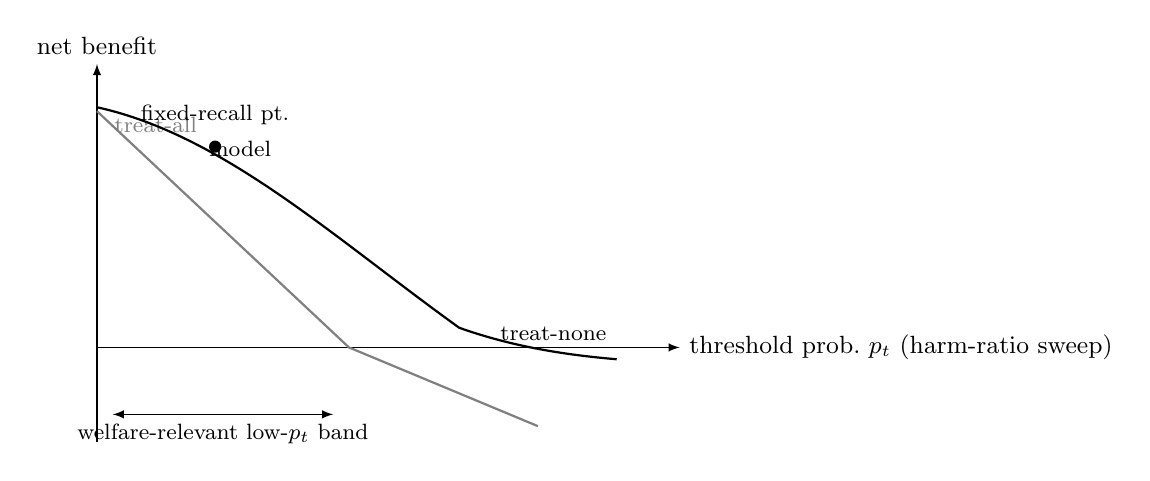
\begin{tikzpicture}[>=latex, font=\small]
% schematic axes only --- NO DATA
\draw[->] (0,0) -- (7.4,0) node[right] {threshold prob.\ $p_t$ (harm-ratio sweep)};
\draw[->] (0,-1.2) -- (0,3.6) node[above] {net benefit};
\draw[dashed] (0,0) -- (7.2,0);
% treat-none baseline (zero net benefit)
\node[font=\footnotesize, anchor=west] at (5.0,0.18) {treat-none};
% treat-all line: high at low pt, crosses to negative
\draw[thick, gray] (0,3.0) -- (3.2,0) -- (5.6,-1.0);
\node[font=\footnotesize, gray, anchor=south west] at (0.1,2.6) {treat-all};
% model curve: dominates over a low-pt band
\draw[thick] (0,3.05) .. controls (1.6,2.7) and (3.0,1.4) .. (4.6,0.25)
  .. controls (5.3,0.0) and (6.0,-0.1) .. (6.6,-0.15);
\node[font=\footnotesize, anchor=south west] at (1.3,2.3) {model};
% annotated fixed-recall point
\fill (1.5,2.55) circle (2.2pt);
\node[font=\footnotesize, anchor=south] at (1.5,2.7) {fixed-recall pt.};
% welfare-relevant band shading marker
\draw[<->] (0.2,-0.85) -- (3.0,-0.85)
  node[midway, below, font=\footnotesize] {welfare-relevant low-$p_t$ band};
\end{tikzpicture}
\caption[Welfare-asymmetric decision curve (schematic)]{\textsc{Schematic
placeholder --- axes and qualitative shape only, no data.} The welfare-asymmetric
decision curve: net benefit versus threshold probability $p_t$, where $p_t$
sweeps the undertreat\,:\,overtreat harm ratio as a range. The headline claim is
that the model curve dominates both treat-all and treat-none across the
welfare-relevant low-$p_t$ band; the fixed-recall operating point is annotated.
The actual curve is to be produced from vet-confirmed held-out scores.}
\label{fig:decision-curve}
\end{figure}

\section{Wrapper Pillar: the fixed pain-recall operating point}
\label{sec:operating-point}

The decision threshold is selected at a \emph{fixed pain-recall} of
$\geq 0.90$ --- the Evangelista sensitivity anchor~\cite{evangelista2019} ---
rather than at a Youden-$J$ or $F_1$ optimum. The selection is performed inside
the training folds only, and the specificity it buys is reported with bootstrap
confidence intervals on out-of-fold predictions. Fixing recall first is the
direct consequence of the welfare asymmetry of \S\ref{sec:decision-curve}: the
dominant cost is missed pain, so the operating point is pinned to control that
miss rate and the specificity cost is reported honestly rather than optimized
against an inappropriate symmetric criterion. This choice corrects the stale
symmetric-knee default and ties the operating point to a clinically meaningful
target. The relevance of a fixed-recall operating point in low-prevalence
settings is sharpened by measurement-error propagation analyses, which show that
modest per-rating error can collapse effective sensitivity when prevalence is
low~\cite{chavoshi2025}; this motivates both the high-recall pin and the
abstention channel of \S\ref{sec:abstention}.

\section{Wrapper Pillar: defer-to-vet abstention as a one-sided NPV lower bound}
\label{sec:abstention}

The abstention pillar reports a defer-to-vet boundary. Around the fixed $0.39$
point, two thresholds $\lambda_1 < \lambda_2$ define a band: confident
no-pain below $\lambda_1$, confident pain above $\lambda_2$, and a deferred
middle band routed to the veterinarian. The reported quantity is the
\emph{negative predictive value} (NPV) --- the dominant clinical cost is a
missed painful cat --- as a function of the abstention rate, and it is reported
as a \textbf{one-sided $95\%$ lower bound at each abstention rate}.

\paragraph{The word ``guaranteed'' is banned.} The lower bound is obtained by a
distribution-free, finite-sample risk-control procedure (Learn-then-Test
\cite{angelopoulos2021ltt}), which controls the NPV risk function at confidence
$\delta = 0.05$ for a tolerated risk $\alpha = 1 - \text{target NPV}$. Because
this is a finite-sample lower bound and not a certainty, the project reports
``NPV with a one-sided $95\%$ lower bound,'' and the word ``guaranteed'' never
appears. Whether a useful band is even certifiable is itself decided by a Gate~0
power calculation \emph{before} any veterinary spend: if the budget cannot
certify NPV $\geq 0.90$ at $\leq 40\%$ abstention, the curve ships
\emph{exploratory-only} and the clinical deliverable relocates to the decision
curve of \S\ref{sec:decision-curve}. This is a demotion, not a kill.

\begin{figure}[t]
\centering
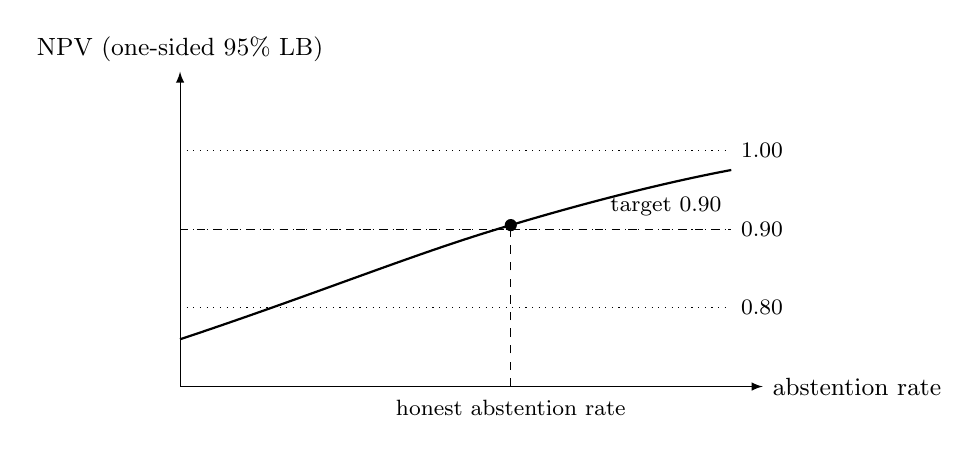
\begin{tikzpicture}[>=latex, font=\small]
% schematic axes only --- NO DATA
\draw[->] (0,0) -- (7.4,0) node[right] {abstention rate};
\draw[->] (0,0) -- (0,4.0) node[above] {NPV (one-sided $95\%$ LB)};
\foreach \y/\l in {1.0/0.80, 2.0/0.90, 3.0/1.00}
  \draw[dotted] (0,\y) -- (7.0,\y) node[right, font=\footnotesize] {\l};
% target line at 0.90
\draw[dashed] (0,2.0) -- (7.0,2.0);
\node[font=\footnotesize, anchor=south east] at (7.0,2.05) {target $0.90$};
% monotone-ish increasing LB curve crossing 0.90 at some honest abstention rate
\draw[thick] (0,0.6) .. controls (1.8,1.2) and (3.0,1.7) .. (4.2,2.05)
  .. controls (5.2,2.35) and (6.2,2.6) .. (7.0,2.75);
% crossing marker
\fill (4.2,2.05) circle (2.2pt);
\draw[dashed] (4.2,0) -- (4.2,2.05);
\node[font=\footnotesize, anchor=north] at (4.2,-0.05) {honest abstention rate};
\end{tikzpicture}
\caption[One-sided NPV lower bound vs.\ abstention rate (schematic)]{\textsc{Schematic
placeholder --- axes and qualitative shape only, no data.} The defer-to-vet
abstention curve: the one-sided $95\%$ NPV lower bound rises with the abstention
rate and clears the $0.90$ target only at an honestly-reported abstention rate.
``Guaranteed'' is never used; the bound is exploratory if the Gate~0 power
budget is unmet. The actual curve is to be produced from vet-confirmed held-out
scores.}
\label{fig:abstention}
\end{figure}

\section{Headline Method 2: the confound-attribution protocol}
\label{sec:confound-protocol}

The second portable contribution is a capture-condition confound-attribution
protocol: a reusable, one-directional audit that any future facial-pain-scorer
corpus can run to ask whether the scorer is reading acquisition context --- the
cage, the clinic, the lighting --- rather than the grimace itself. Single-source
data makes this audit essential: pain and capture condition are plausibly
entangled, and a scorer that exploits that entanglement would post strong
accuracy while learning nothing about pain. The deliverable is the
\emph{protocol}, released as code, not a verdict about this particular corpus.

\paragraph{One-directional by construction.} The audit is well-powered to
\emph{detect} confounding but underpowered to \emph{rule it out}. Every report
therefore reads ``no confound detected at this power'' --- never ``no
confound.'' This asymmetry is stated as a fixed property of the method, not a
caveat appended after the fact.

The protocol has two components, summarized in Figure~\ref{fig:confound}.

\paragraph{(a) FGS-BG-Gap --- the background counterfactual.} The cat face is
masked (training-free, via DINOv2 attention rollout, a segment-anything mask, or
grabcut) and composited onto (i) a same-condition and (ii) a \emph{swapped}
clinic background; the score shift is measured. FGS-BG-Gap is reported as the
mean $0$--$10$ shift plus the pain-flip rate, per AU, stratified by capture
condition. A large gap on a specific AU indicates that head is reading the
cage or clinic rather than the cat. This component adapts the
background-robustness counterfactual framework~\cite{xiao2021background} to the
FGS setting.

\paragraph{(b) Per-AU EBPG --- the energy-based pointing game.} Per-AU saliency
(attention rollout or Score-CAM~\cite{wang2020scorecam} on the frozen backbone)
is scored against an anatomical region of interest derived from CatFLW
landmarks: the protocol reports $\text{energy-in-ROI} / \text{energy-whole}$ per
AU, stratified by capture condition. This answers the question ``does the ear
head fire on the ear?'' --- a per-AU localization-faithfulness measurement that
no prior cat-pain work reports. Where landmark coverage is partial, EBPG is
reported only on the covered subset with the denominator stated.

\begin{figure}[t]
\centering
\begin{tikzpicture}[
  node distance=6mm and 12mm,
  box/.style={draw, rounded corners, align=center, inner sep=4pt, font=\small},
  outbox/.style={draw, align=center, inner sep=4pt, font=\footnotesize, fill=black!6},
  oned/.style={draw, dashed, align=center, inner sep=3pt, font=\footnotesize},
  >=latex
]
\node[box] (face) {face crop\\+ AU saliency\\+ landmarks};
% branch A
\node[box, above right=4mm and 20mm of face] (mask) {mask face,\\swap clinic\\background};
\node[outbox, right=of mask] (bggap) {FGS-BG-Gap\\$=\overline{|\Delta\,\text{sum}|}$\\+ pain-flip rate, per AU};
% branch B
\node[box, below right=4mm and 20mm of face] (sal) {per-AU saliency\\vs.\ CatFLW\\AU ROI};
\node[outbox, right=of sal] (ebpg) {per-AU EBPG\\$=\dfrac{\text{energy-in-ROI}}{\text{energy-whole}}$};
\node[oned, right=14mm of bggap, yshift=-9mm] (report)
  {report stratified by capture condition:\\\textbf{``no confound detected at this power''}\\(one-directional)};

\draw[->] (face) -- (mask);
\draw[->] (face) -- (sal);
\draw[->] (mask) -- (bggap);
\draw[->] (sal) -- (ebpg);
\draw[->] (bggap.east) -- (report.west);
\draw[->] (ebpg.east) -- (report.west);
\end{tikzpicture}
\caption[Confound-attribution protocol]{The capture-condition
confound-attribution protocol (Headline Method~2), portable and
one-directional. Branch (a) FGS-BG-Gap measures the score shift under a swapped
clinic background; branch (b) per-AU EBPG measures whether each AU head's
saliency falls inside its anatomical ROI. Both are stratified by capture
condition and reported as ``no confound detected at this power.'' The deliverable
is the protocol, not a verdict on any single corpus.}
\label{fig:confound}
\end{figure}

\section{Where calibration sits: supporting evidence, never headline}
\label{sec:calibration-supporting}

For completeness, the $0$--$10$ layer's reliability is examined through the
distributional decode path of the engine (soft cumulative probabilities $\to$
per-AU probability mass functions $\to$ convolution to a $0$--$10$ sum pmf),
yielding a ranked probability score on the sum and per-AU classwise expected
calibration error~\cite{guo2017calibration}. These calibration quantities are
\emph{supporting evidence only}. They are never a headline; no binned
reliability diagram is drawn on the degenerate $11$-atom sum; and they never
substitute for the welfare-asymmetric decision curve of
\S\ref{sec:decision-curve}, which remains the headline wrapper artifact. This
keeps the contribution clearly located in the two portable methods and the
welfare framing, with generic calibration relegated to hygiene.

\section{Summary}
\label{sec:ch5-summary}

This chapter specified the supervision and trustworthiness layers that carry the
project's contribution. The VLM weak-labeler emits five rationale-before-score
ordinal atoms under a forced-tool-use enum contract, with the sum and the $0.39$
flag computed in code so the labeler never makes a clinical decision. Headline
Method~1 measures per-AU VLM-versus-vet quadratic-weighted kappa, gated on the
CI lower bound; Headline Method~2 is a one-directional, portable
confound-attribution protocol. Between them, a welfare-asymmetric decision
curve, a fixed pain-recall operating point, and a one-sided NPV-lower-bound
abstention boundary constitute the clinical frame, while the circularity
firewall ensures that validation rides on vet-confirmed labels only and that
agreement-against-VLM is never mistaken for validation. The engine remains
conceded plumbing; the contribution lives here, and every claim in this chapter
is stated as a protocol and a decision rule, not as a result.
